\documentclass[12pt, a4paper]{article}
\usepackage{enumitem}
\usepackage{float}
\usepackage[left=2cm, right=2cm, top=2cm, bottom=2cm]{geometry}
\usepackage{graphicx}
\usepackage{tabularx}
\usepackage{xeCJK}

\renewcommand\arraystretch{1.1}
\setCJKmainfont[AutoFakeBold=1.5]{新細明體}

\newcommand*{\var}[1]{{\itshape\verb|#1|}}

\setlist{%
  itemsep=0pt
}

\title{%
  \vspace{-1.5cm}
  Systems Programming (2024 Fall)\\
  Programming Assignment 2
}
\author{\Large B12902110 呂承諺}
\date{}

\begin{document}
  \maketitle

  \section{I/O and file descriptors}
  The following table shows the file descriptors that a process uses to communicate
  to the outside, its parent, or its children.
  \begin{table}[H]
    \centering
    \caption{File descriptors and their usages}
    \begin{tabular}{|c|c|c|}
      \hline
      \textbf{fd} & \textbf{Root} & \textbf{Non-root nodes} \\\hline
      0 & Input from outside (command) & Input from parent (command) \\\hline
      1 & \multicolumn{2}{c|}{Output to outside (answer)} \\\hline
      2 & \multicolumn{2}{c|}{Output to outside (debug messages)} \\\hline
      3 & \verb|/dev/null| & Output to parent (response) \\\hline
      4,5,\dots & \multicolumn{2}{c|}{Pipe I/O to and from children, or FIFOs} \\\hline
    \end{tabular}
  \end{table}

  In this project, we use the standard I/O functions from the C library, and open
  every file descriptor as a stream either with \verb|fopen()| or \verb|fdopen()|.
  Every stream is set to unbuffered mode to avoid issues.

  \section{Main logic}
  \subsection{Initialization}
  When a node is created, i.e., \verb|friend| is executed, it performs the
  following initialization procedures.
  \begin{enumerate}
    \item Sets global variables \verb|current_info|, \verb|current_name|,
    \verb|current_value|, and \verb|is_root| according to \verb|argv[1]|.
    \item Opens \verb|parent_write_stream| (corresponds to fd 3) for writing response to parent.
    For the root note, this stream will write to \verb|/dev/null|.
    \item Initialize the \verb|children| array with \verb|InitializeFriend()|.
  \end{enumerate}

  \subsection{Command dispatching}
  Then the node keeps listening for commands on stdin (fd 0), which for the root
  is from the outside and for all other nodes is from the parent.
  Depending on whether the command's \textit{target node} is the current node or not, we
  either handle the command or relay the command to our children, by calling the
  corresponding handler or relay function respectively.
  Note that some commands require a lot of stuff done at the root node; in that case,
  we call the special root handler for that command if we're at the root node.

  \begin{table}[H]
    \centering
    \caption{Handler and relay functions for each command}
    \begin{tabular}{|c|c|c|c|}
      \hline
      \textbf{Command} & \textbf{Handler function} & \textbf{Relay function} & \textbf{Special root handler function}\\\hline
      \multicolumn{4}{|c|}{Public commands} \\\hline
      Meet & \verb|HandleMeet()| & \verb|RelayMeet()| & N/A \\\hline
      Check & \verb|HandleCheck()| & \verb|RelayCheck()| & N/A \\\hline
      Graduate & \verb|HandleGraduate()| & \verb|RelayGraduate()| & A few lines in \verb|main()| \\\hline
      Adopt & \verb|HandleAdopt()| & \verb|RelayAdopt()| & \verb|RootHandleAdopt()| \\\hline
      Compare & \verb|HandleCompare()| & \verb|RelayCompare()| & \verb|RootHandleCompare()| \\\hline
      \multicolumn{4}{|c|}{Internal commands} \\\hline
      LevelPrint & \verb|HandleLevelPrint()| & \verb|RelayPrint()| & N/A \\\hline
      Search & \verb|HandleSearch()| & \verb|RelaySearch()| & N/A \\\hline
      AdoptPrint & \verb|HandleAdoptPrint()| & \verb|RelayAdoptPrint()| & N/A \\\hline
      CompareMod & \verb|HandleCompareMod()| & N/A & N/A \\\hline
    \end{tabular}
  \end{table}
  \begin{table}[H]
    \centering
    \caption{Condition for determining whether to handle the command}
    \begin{tabular}{|c|c|}
      \hline
      \textbf{Command} & \textbf{Condition for handling} \\\hline
      \multicolumn{2}{|c|}{Public commands} \\\hline
      Meet & \verb|current_name == parent_friend_name| \\\hline
      Check & \verb|current_name == parent_friend_name| \\\hline
      Graduate & \verb|current_name == friend_name| \\\hline
      Adopt & \verb|is_root| / \verb|current_name == parent_friend_name| \\\hline
      Compare & \verb|is_root| / \verb|current_name == friend_name| \\\hline
      \multicolumn{2}{|c|}{Internal commands} \\\hline
      LevelPrint & \verb|level == 0| \\\hline
      Search & \verb|current_name == parent_friend_name| \\\hline
      AdoptPrint & \verb|current_name == child_friend_name| \\\hline
      CompareMod & Always (No need to relay) \\\hline
    \end{tabular}
  \end{table}

  The following figure illustrates the dependency relationships between each command.\nopagebreak
  \begin{figure}[H]
    \centering
    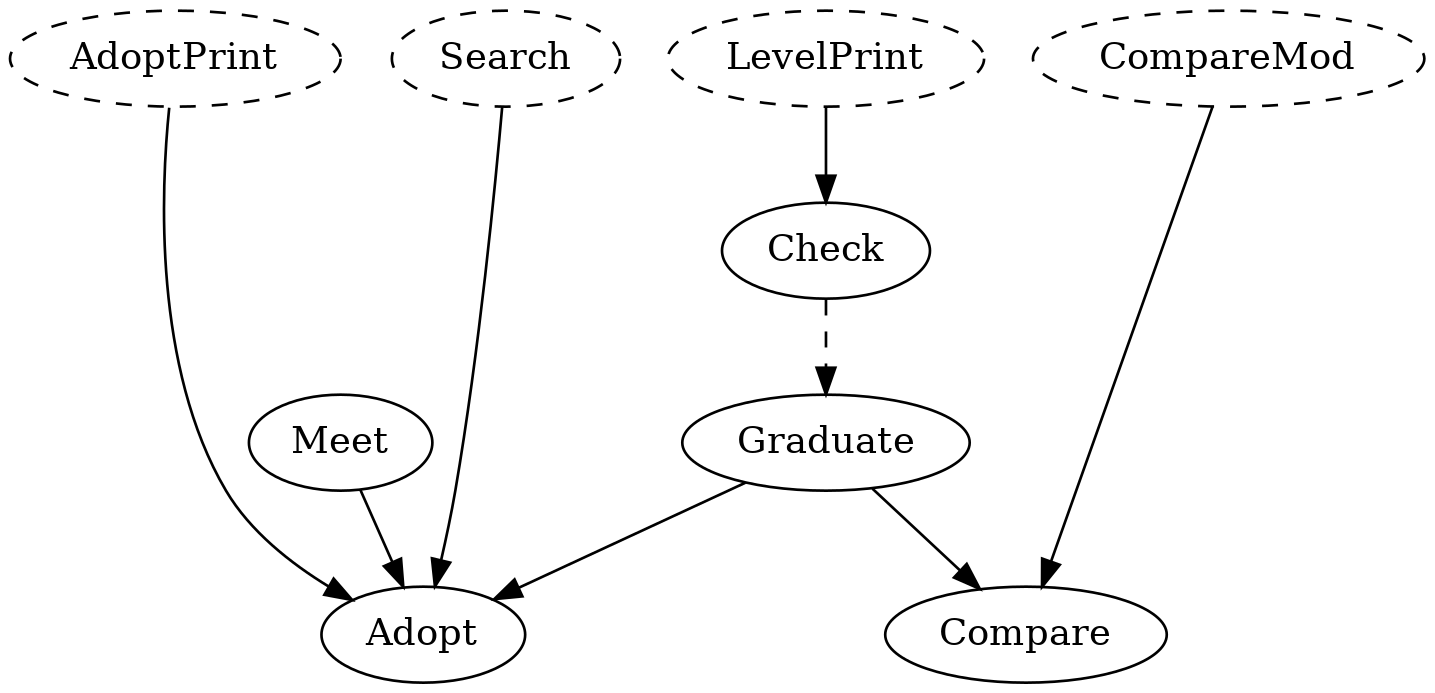
\includegraphics[width=0.7\linewidth]{command_dependency.png}
    \caption{Dependency relationships between each command}
  \end{figure}

  \subsection{Interprocess communication}
  The key idea is to use interprocess communication (IPC) to simulate depth-first search (DFS)
  and pre-order traversal on the tree. Sending a command to a child is like calling
  a function, and sending a response back to the parent is like returning from a function.
  DFS is crucial for this project, as it is used by all of the relay functions
  and some of the handler functions.

  The table below shows the possible response codes that a node could send to
  its parent. They are implemented as type \verb|response_t|.
  \begin{table}[H]
    \centering
    \caption{Response codes}
    \begin{tabularx}{\linewidth}{|l|X|}
      \hline
      \multicolumn{1}{|c|}{\textbf{Response code}} &
      \multicolumn{1}{c|}{\textbf{Description}}
      \\\hline
      \verb|REPSONSE_HANDLE_OK| &
      The current node has successfully handled the command.
      \\\hline
      \verb|RESPONSE_RELAY_OK| &
      The current node has successfully relayed the command. That is, one of the
      node's descendants has successfully handled the command.
      \\\hline
      \verb|RESPONSE_RELAY_OK_NO_PRINT| &
      Only used in the LevelPrint command. A special instance of
      \verb|RESPONSE_RELAY_OK|, indicting nothing is printed at the target level
      for the subtree rooted at the current node.
      We need this to handle spaces and newlines for the Check command.
      \\\hline
      \verb|RESPONSE_NOT_FOUND| &
      The target node for handling the command is not in the subtree of the
      current node, so we have to keep DFS-ing for the target node.
      \\\hline
      \verb|RESPONSE_SEARCH_FOUND| &
      Only used in the Search command. The search target is found in the subtree of
      the current node.
      \\\hline
      \verb|RESPONSE_SEARCH_FOUND| &
      Only used in the Search command. The search target is not found in the subtree of
      the current node.
      \\\hline
      \verb|RESPONSE_EMPTY| &
      An error has occurred.
      \\\hline
      \end{tabularx}
  \end{table}

  For the \textit{relay} family of functions, their primary purpose is to
  DFS for the \textit{target node} who is responsible for handling the command.
  Therefore, they send the command (mostly) as is to its children one at a time,
  and then wait for a response.
  If the response is either \verb|RESPONSE_HANDLE_OK| or \verb|RESPONSE_RELAY_OK|,
  we respond \verb|RESPONSE_RELAY_OK| to the parent and end the search. This
  forms a relay chain back to the root node. Otherwise, we continue searching.

  Some commands requires additional work to be done in the relay family of functions,
  such as Graduate, AdoptPrint, and CompareMod.
  For Graudate, it's because the target's parent need to wait for the target
  to die; for AdoptPrint and CompareMod, it's because they need access to the
  \verb|children| array or name of the target's parent.

  On the other hand, the \textit{handler} family of functions are those
  who actually access the tree. Some handler functions also recursively
  dispatch the command to descendants and gather the results.

  The return value for the handler and relay functions will be returned to
  \verb|main()|, which subsequently will be the response code sent to the parent.
  Note that the root node has fd 3 opened at \verb|/dev/null|; this means that
  any response the root node tries to send to its parent will be discarded, as
  there is no parent node by definition.

  \pagebreak
  However, there are two special scenarios that doesn't use this mechanism:\nobreak
  \begin{enumerate}
    \item Due to blocking I/O constraints regarding FIFOs, the Compare command
    requires responses be sent early in the handler function and the response mechanism
    in \verb|main()| be suppressed. Here we use the \verb|close()| of FIFOs as
    the response mechanism.

    For more information, see the implementation of \verb|HandleAdopt()| and
    \verb|HandleCompare()|.

    \item For the handler part of Graduate, we use \verb|waitpid()| as the response
    mechanism.
  \end{enumerate}

  In conclusion, a command sent to a child is always paired with a response
  from that child, except Graduate.
  The response code is analogous to the return status of a function call.

  \section{Custom commands}
  Now we explain the usages and functionalities of custom commands.
  \subsection{Internal commands}
  The internal commands should only be invoked from nodes and never
  from the outside.
  \begin{table}[H]
    \centering
    \caption{Internal commands}
    \begin{tabularx}{\linewidth}{|c|l|X|}
      \hline
      \textbf{Command} &
      \multicolumn{1}{c|}{\textbf{Usage}} &
      \multicolumn{1}{c|}{\textbf{Description}}
      \\\hline
      LevelPrint &
      \texttt{L \var{LEVEL} \var{HAS_PRINTED}} &
      Print all nodes that are \var{LEVEL} levels deeper than the current node.
      \var{HAS_PRINTED} is a flag denoting whether anything about the target
      level has been printed.
      \\\hline
      Search &
      \texttt{S \var{PARENT} \var{CHILD}} &
      Search for \var{CHILD} under the subtree of \var{PARENT}. Essentially
      Check without printing.
      \\\hline
      AdoptPrint &
      \texttt{P \var{CHILD}} &
      Recursively print all parent-child relationships in the current subtree
      to file \verb|Adopt.fifo|.
      \\\hline
      CompareMod &
      \texttt{\%} &
      Recursively let all descendants have their \texttt{(friend\_value * 2) \% 99}.
      \\\hline
    \end{tabularx}
  \end{table}

  \subsection{Extensions to public commands}
  \subsubsection{Meet}
  There are two variations of the Meet command, \verb|Meet| and \verb|meet|.
  \verb|Meet| follows the description in the problem spec. \verb|meet| is
  exactly the same as \verb|Meet|, except that it suppress output, which is
  used in the Adopt command for creating new nodes.
  For more information, see \verb|HandleMeet()| and \verb|HandleAdopt()|.
  \subsubsection{Adopt}
  There are two variations of the Adopt command, \verb|Adopt| and \verb|adopt|.
  \verb|adopt|, with a lowercase \verb|a|, only opens the read end of
  \verb|Adopt.fifo| in nonblocking mode, so that the AdoptPrint command can open
  the write end of \verb|Adopt.fifo|.
  After all the information needed for adoption is in the FIFO, \verb|Adopt|,
  with an uppercase \verb|A|, is the one that actually reads the information and
  issues the Meet commands.

  The adopt relay and handler functions accept a parameter \verb|op|
  of type \verb|adopt_op_t|, representing either one of ``open mode" or ``read
  mode". For more information, see \verb|HandleAdopt()|.

  \section{Command implementations}
  \subsection{Meet}
  \subsubsection{Relay}
  \begin{itemize}
    \item \textbf{Command passing}: As is.
    \item \textbf{Output}: If the target node is not found, output the corresponding answer.
  \end{itemize}

  \subsubsection{Handler}
  The parent friend for Meet does the following operations.
  \begin{enumerate}
    \item Prepare two pipes to communicate with it, one for reads and one for writes.
    \item \verb|fork()| a new process and \verb|exec()| \verb|./friend <child_friend_info>|.
    \item Add an \verb|Friend| entry in the \verb|children| array.
    \item Output answer response to outside.
  \end{enumerate}

  \subsection{Check}
  \subsubsection{Relay}
  \begin{itemize}
    \item \textbf{Command passing}: As is.
    \item \textbf{Output}: If the target node is not found, output the corresponding answer.
  \end{itemize}

  \subsubsection{Handler}
  The root node of the subtree to be printed does the following operations.
  \begin{enumerate}
    \item Print the current node's information.
    \item Run the LevelPrint command, which tells nodes that are 1 to
    \verb|MAX_TREE_DEPTH| levels deeper than the current node to print their
    information, one level at a time, separated by a newline.
    In fact, this is iterative deepening depth-first search (IDFFS).
  \end{enumerate}

  \subsection{Graduate}
  \subsubsection{Root handler (a few lines in \texttt{main()})}
  Run Check first. If the target is not found, output the corresponding answer
  and end this command.

  \subsubsection{Relay}
  \begin{itemize}
    \item \textbf{Command passing}: As is.
    \item \textbf{Output}: No output.
    \item \textbf{Special work when child is target}: Wait for it to die, and clean up
    it's entry in the \verb|children| array, including closing pipe file descriptors that
    were used to communicate with it.
    \item \textbf{Special response mechanism}: If the child node is the target node,
    use \verb|waitpid()| as the response mechanism. Otherwise use the normal
    response codes.
  \end{itemize}

  \subsubsection{Handler}
  The root node of the subtree to be removed does the following operations.
  \begin{enumerate}
    \item Recursively send the Graduate command to each child. and wait for them
    to die with \verb|waitpid()|. A child is dead implies its whole subtree is
    dead.
    \par\textbf{Special response mechanism}: Wait for a child to die with \verb|waitpid()|.
    \item Terminate the current process with \verb|_exit()|.
  \end{enumerate}

  \subsection{Adopt}
  This command's target node is the adopting parent. In contrast, the target
  node of the AdoptPrint command is the root node of the subtree to be aodpted.

  \subsubsection{Root handler (a few lines in \texttt{main()})}
  At the root node, do the following operations.
  \begin{enumerate}
    \item Run ``\verb|Search child_friend_name parent_friend_name|" to determine if the
    subtree to be adopted is a descendant of the adopting node.
    If yes, output the corresponding answer and end this command.
    \item Create \verb|Adopt.fifo| with \verb|mkfifo()|.
    \item Run the Adopt command in \verb|ADOPT_OPEN| mode.
    Let the adopting node
    \item Run the AdoptPrint command. This will print every parent-child
    information about the subtree to be adopted into the FIFO.
    \item Graduate the original subtree that is about to be adopted.
    \item Run the Adopt command in \verb|ADOPT_READ| mode.
    \item Remove the FIFO with \verb|unlink()|.
  \end{enumerate}

  \subsubsection{Relay}
  \begin{itemize}
    \item \textbf{Command passing}: As is.
    \item \textbf{Output}: No output.
  \end{itemize}

  \subsubsection{Handler}
  The root node of the subtree to be adopted does the following operations.

  \medskip
  \noindent \verb|ADOPT_OPEN| \textbf{mode}: Open the read end of the FIFO in nonblocking mode.

  \medskip
  \noindent \verb|ADOPT_MODE| \textbf{mode}:
  \begin{enumerate}
    \item Read all contents in the FIFO and run Meet command for each parent-child
    relationship.
    \item Close the FIFO.
  \end{enumerate}

  \subsection{Compare}
  \subsubsection{Root handler}
  The root node does the following operations.
  \begin{enumerate}
    \item Create the two FIFOs with \verb|mkfifo()|.
    \item Pass down the compare command to the target node to be compared, so that it can
    open the read end of \verb|number.fifo|.
    \item Open the write end of \verb|number.fifo| and write \verb|number|
    to it.
    \item Open the read end of \verb|<friend_name>.fifo| and read the compare outcome.
    \par\textbf{Special response mechanism}: This step should block until the response can be
    read, so we use this as the response mechanism.
    \item According to the compare outcome, output the corresponding answer message.
    \par If the compare outcome is \verb|COMPARE_GRADUATE|, run
    ``\verb|Graduate friend_name|" to remove the subtree.
    \item Close and remove the two FIFOs.
  \end{enumerate}

  \subsubsection{Relay}
  \begin{itemize}
    \item \textbf{Command passing}: As is.
    \item \textbf{Output}: No output.
    \item \textbf{Special work when child is target}: Modify the value and info of
    the child's entry in the \verb|children| array.
  \end{itemize}

  \subsubsection{Handler}
  The target node that is compared with performs the following operations.
  \begin{enumerate}
    \item Early respond so that the root node can write the number to \verb|number.fifo|.

    \textbf{Special response mechanism}: We use the blocking of
    \verb|<friend_name>.fifo| as the response mechanism for this command.
    \item Open the read end of \verb|number.fifo| and read from it.
    \item Compare the number read from \verb|number.fifo| and write the
    compare outcome to\\
    \verb|<friend_name>.fifo|.
    \item Compare the number to the current node's value and write the output
    to the response FIFO.
    \par If the outcome is \verb|COMPARE_MOD|, run CompareMod to have all
    descendants have their value modded.
    \item Close the two FIFOs.
  \end{enumerate}

  \subsection{Internal commands}
  The implementation details for internal commands are omitted for brevity.

\end{document}
